\chapter{Comparison of Data with Background Events}
\label{databackgroundapp}

\subsection{Comparison of Muon Data Events with Expectation}

\subsubsection{Leading Jet P$_{T}$}

\begin{figure}[!h!tbp]
\begin{center}
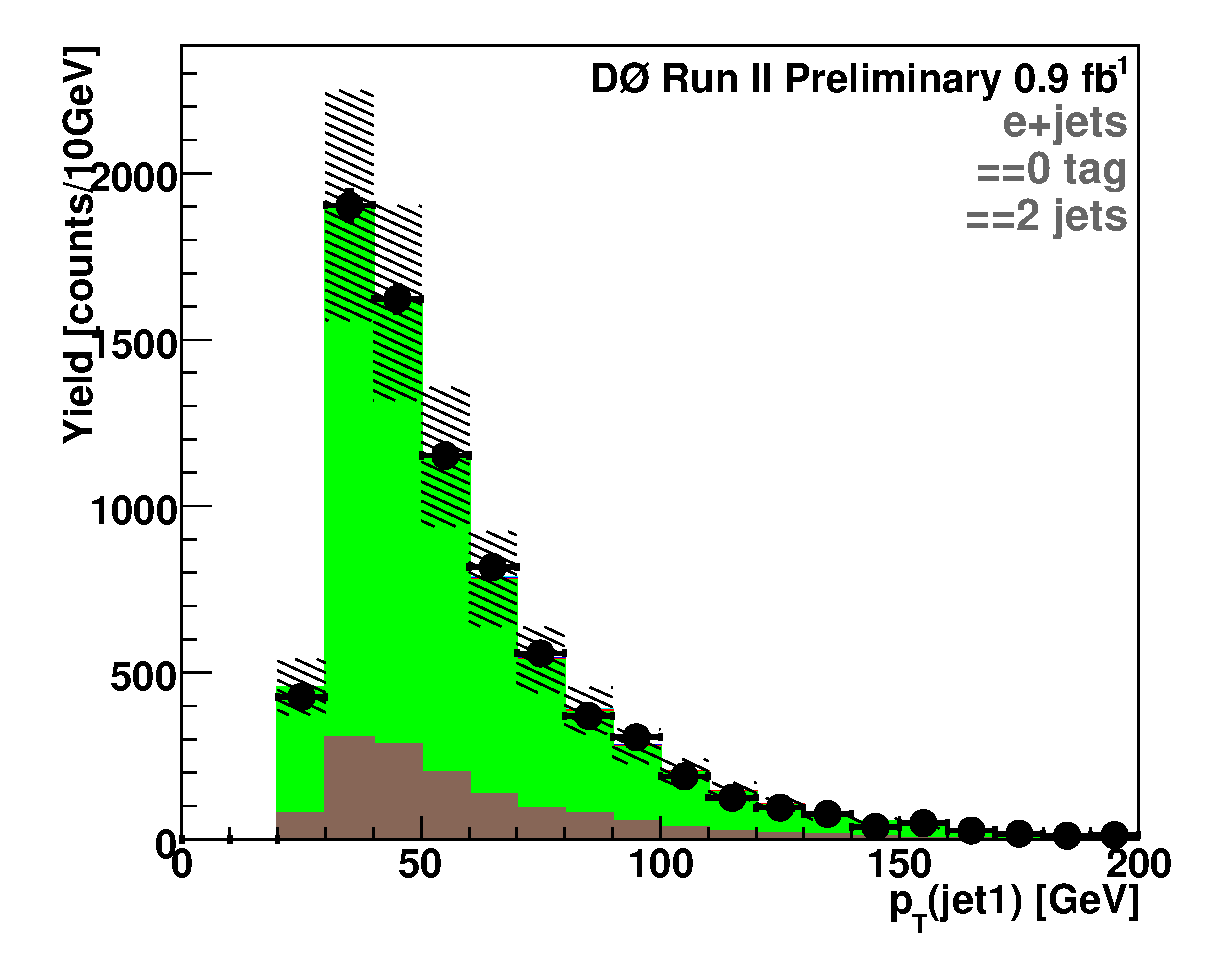
\includegraphics[width=0.32\textwidth]{eps/DataBackground/electron/CC_EqZeroTag_EqTwoJet_Jet1Pt.eps}
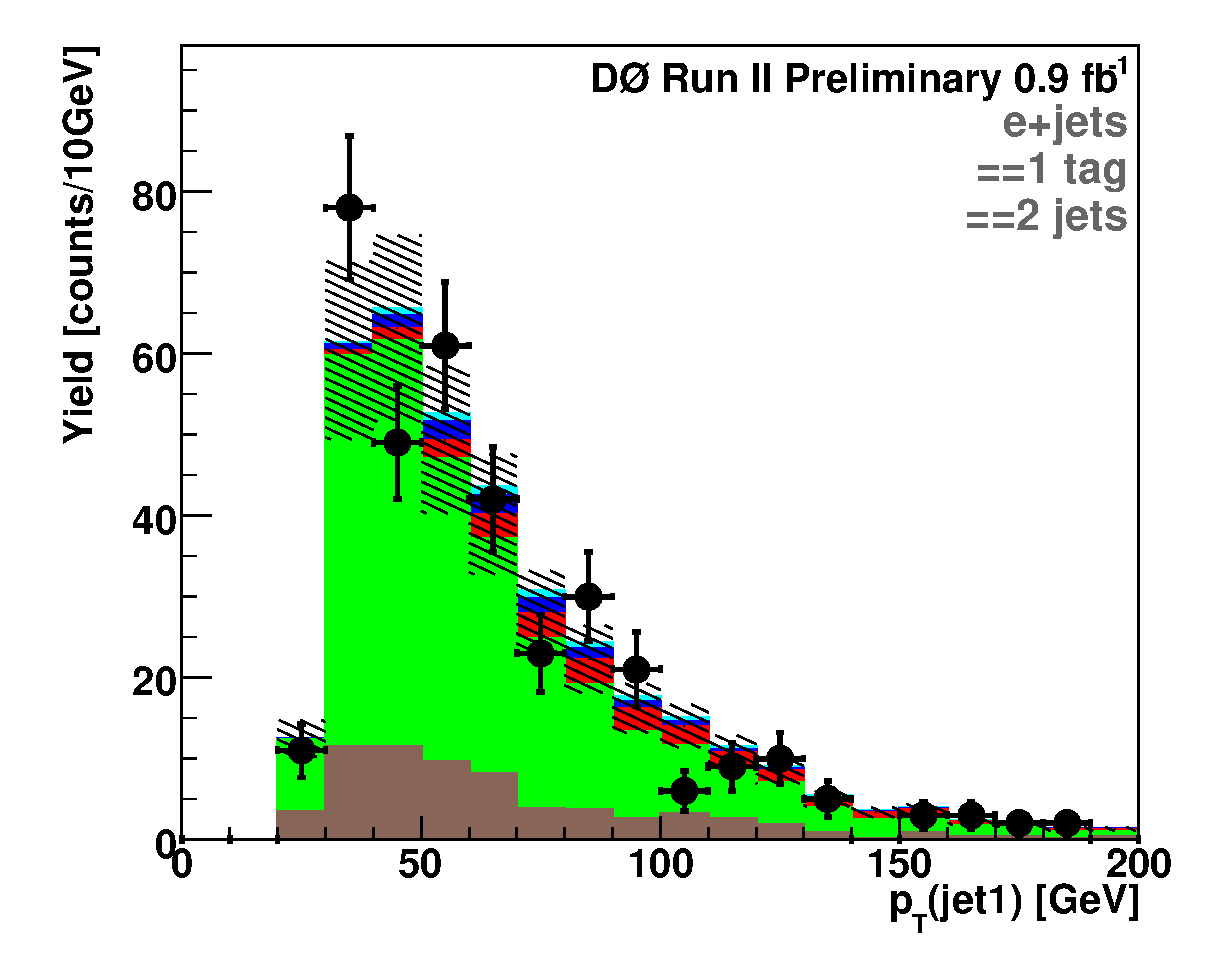
\includegraphics[width=0.32\textwidth]{eps/DataBackground/electron/CC_EqOneTag_EqTwoJet_Jet1Pt.eps}
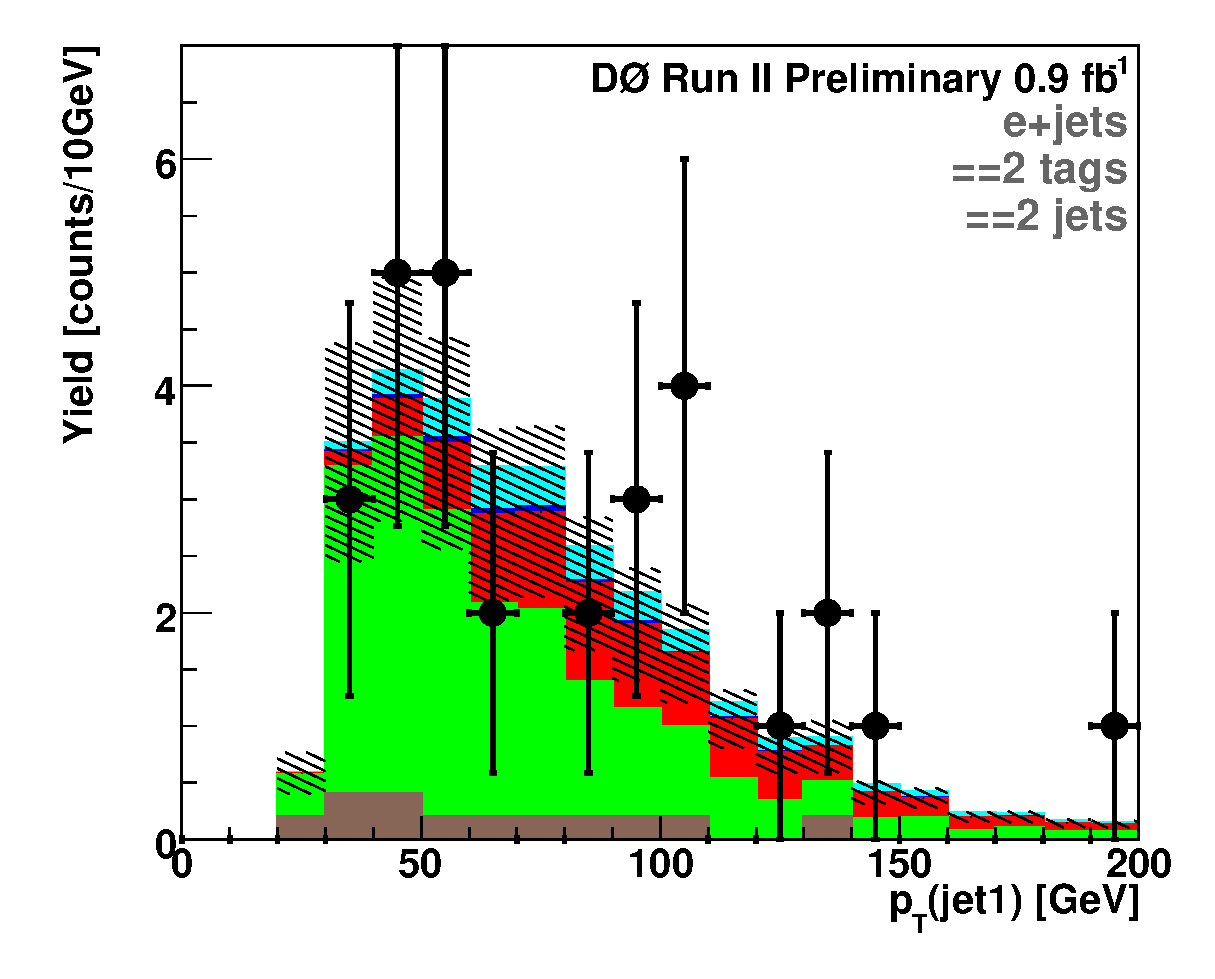
\includegraphics[width=0.32\textwidth]{eps/DataBackground/electron/CC_EqTwoTag_EqTwoJet_Jet1Pt.eps}
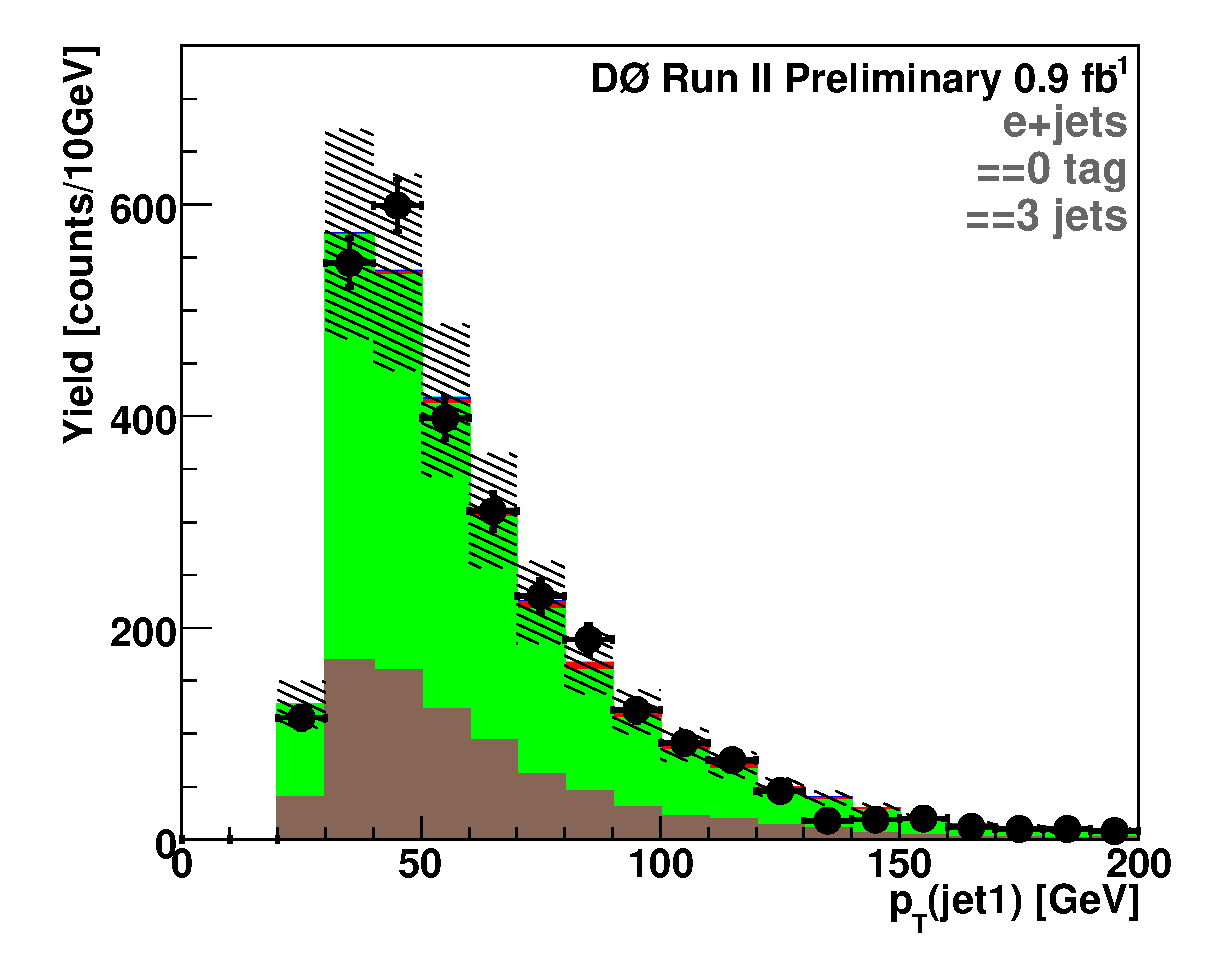
\includegraphics[width=0.32\textwidth]{eps/DataBackground/electron/CC_EqZeroTag_EqThreeJet_Jet1Pt.eps}
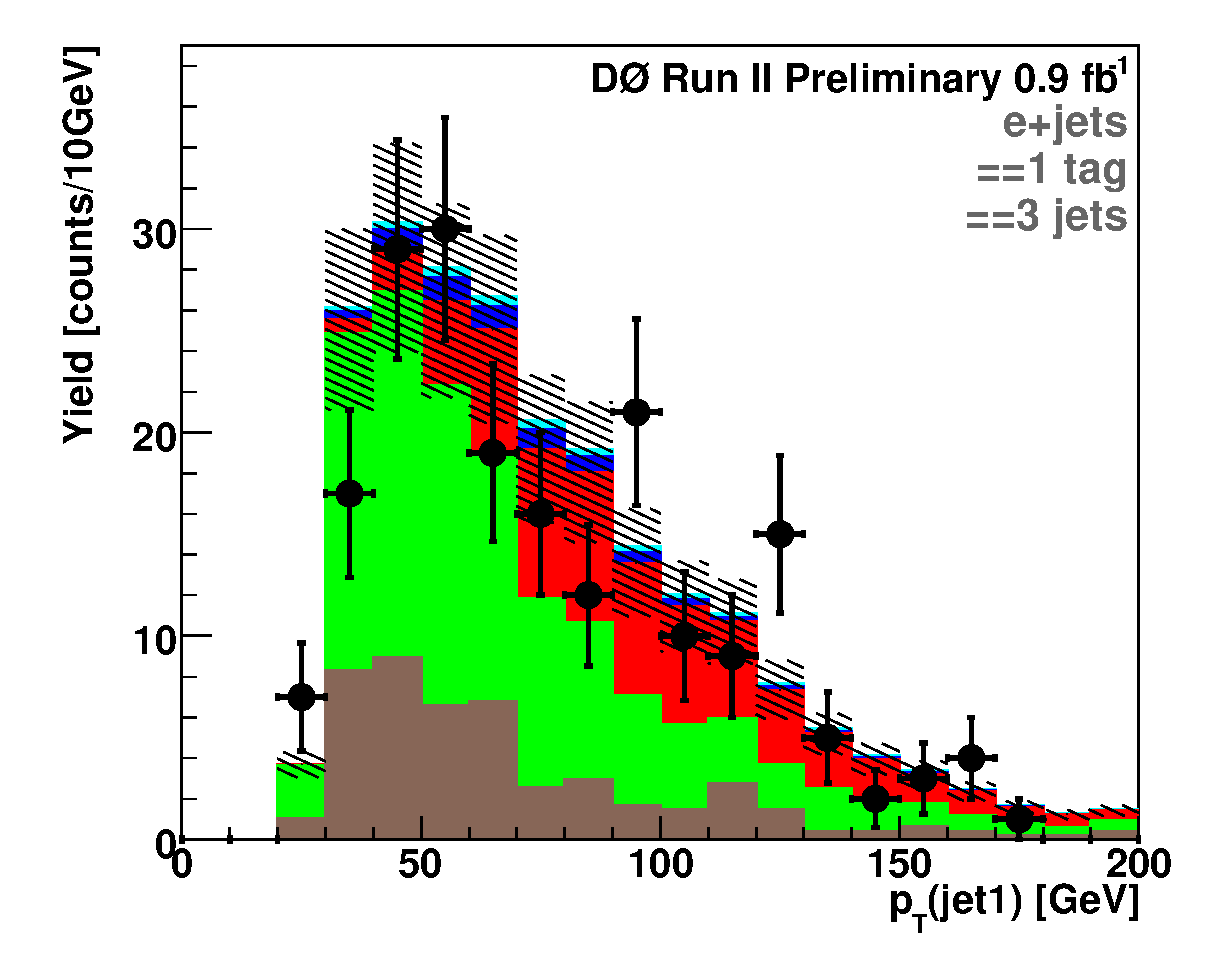
\includegraphics[width=0.32\textwidth]{eps/DataBackground/electron/CC_EqOneTag_EqThreeJet_Jet1Pt.eps}
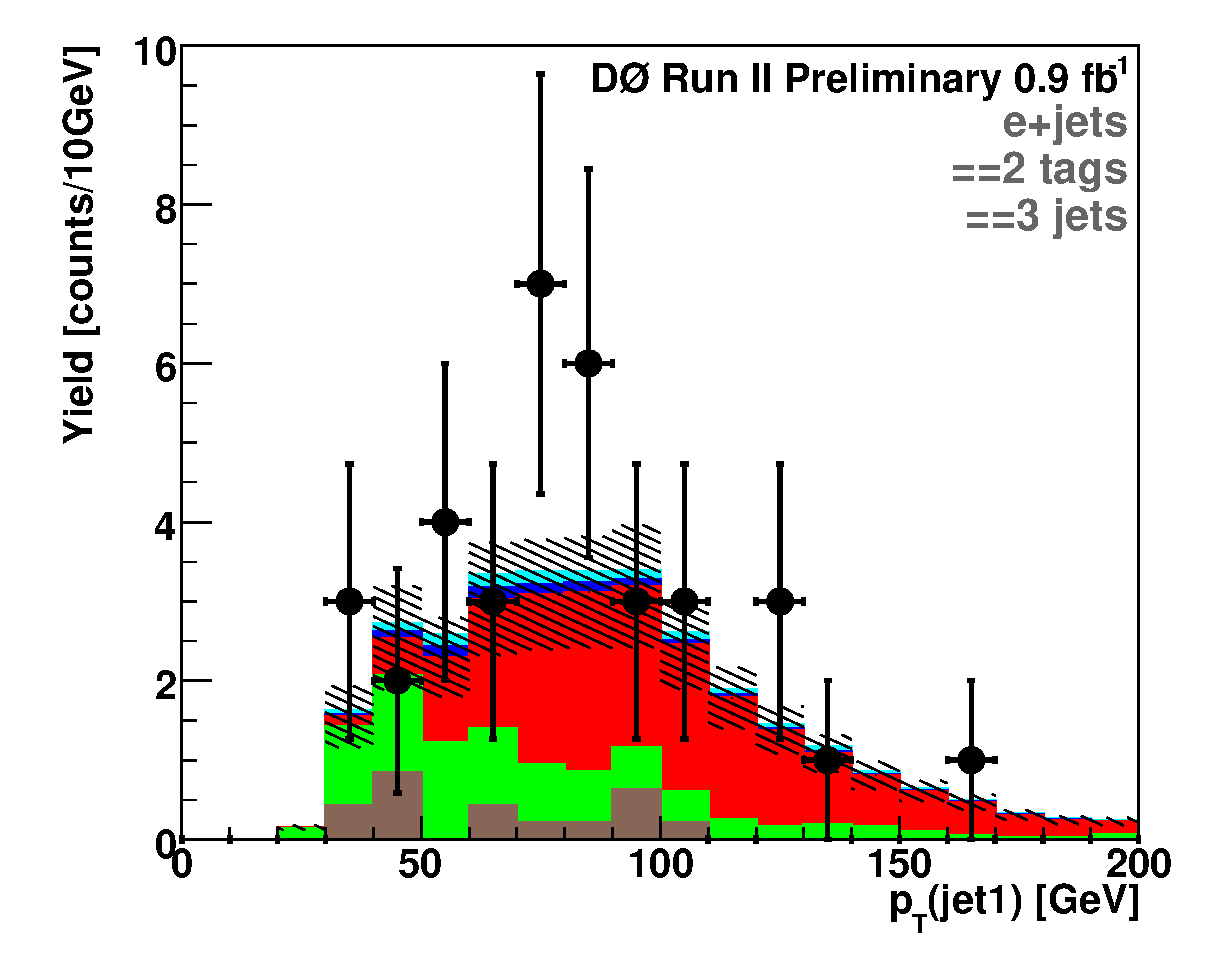
\includegraphics[width=0.32\textwidth]{eps/DataBackground/electron/CC_EqTwoTag_EqThreeJet_Jet1Pt.eps}
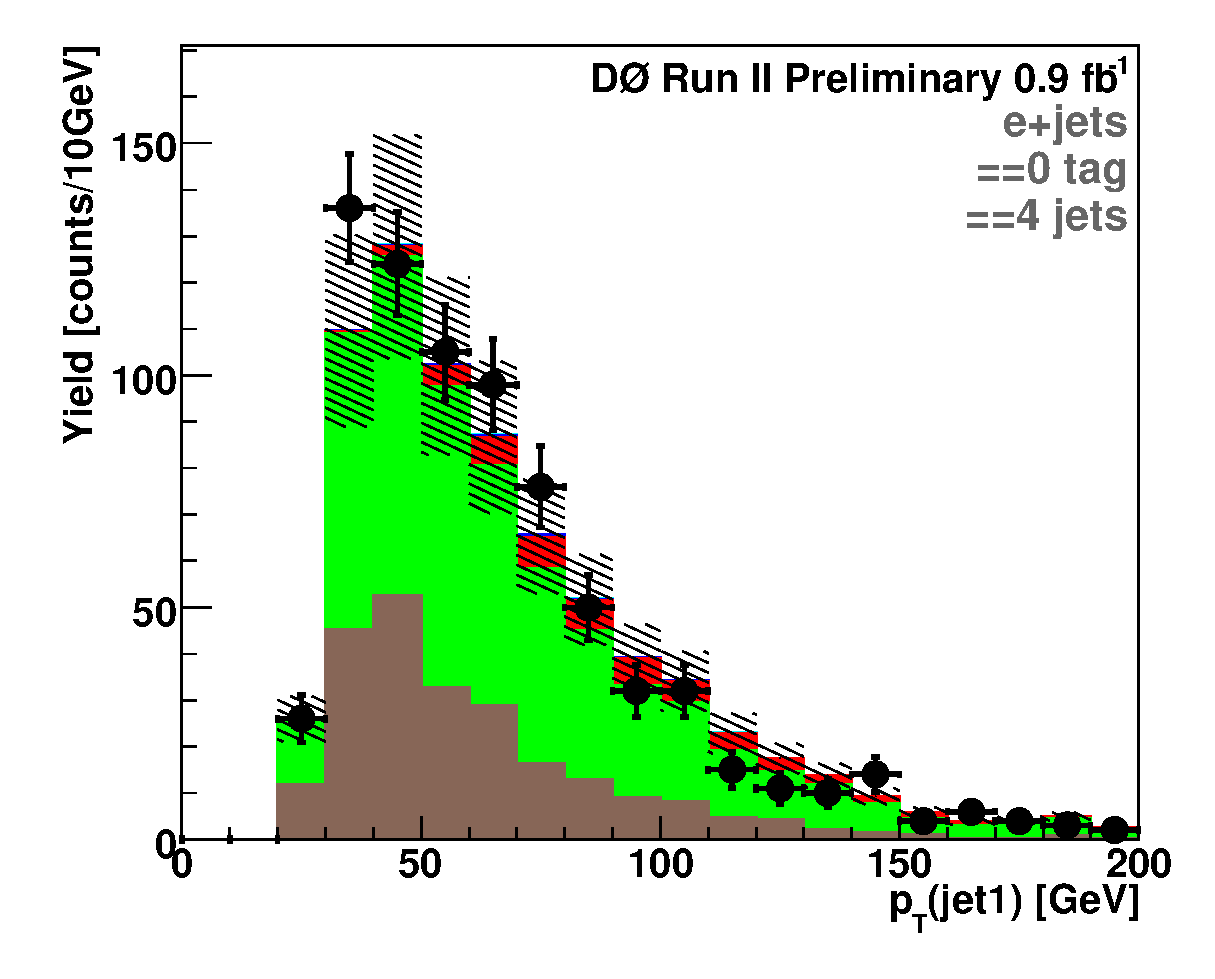
\includegraphics[width=0.32\textwidth]{eps/DataBackground/electron/CC_EqZeroTag_EqFourJet_Jet1Pt.eps}
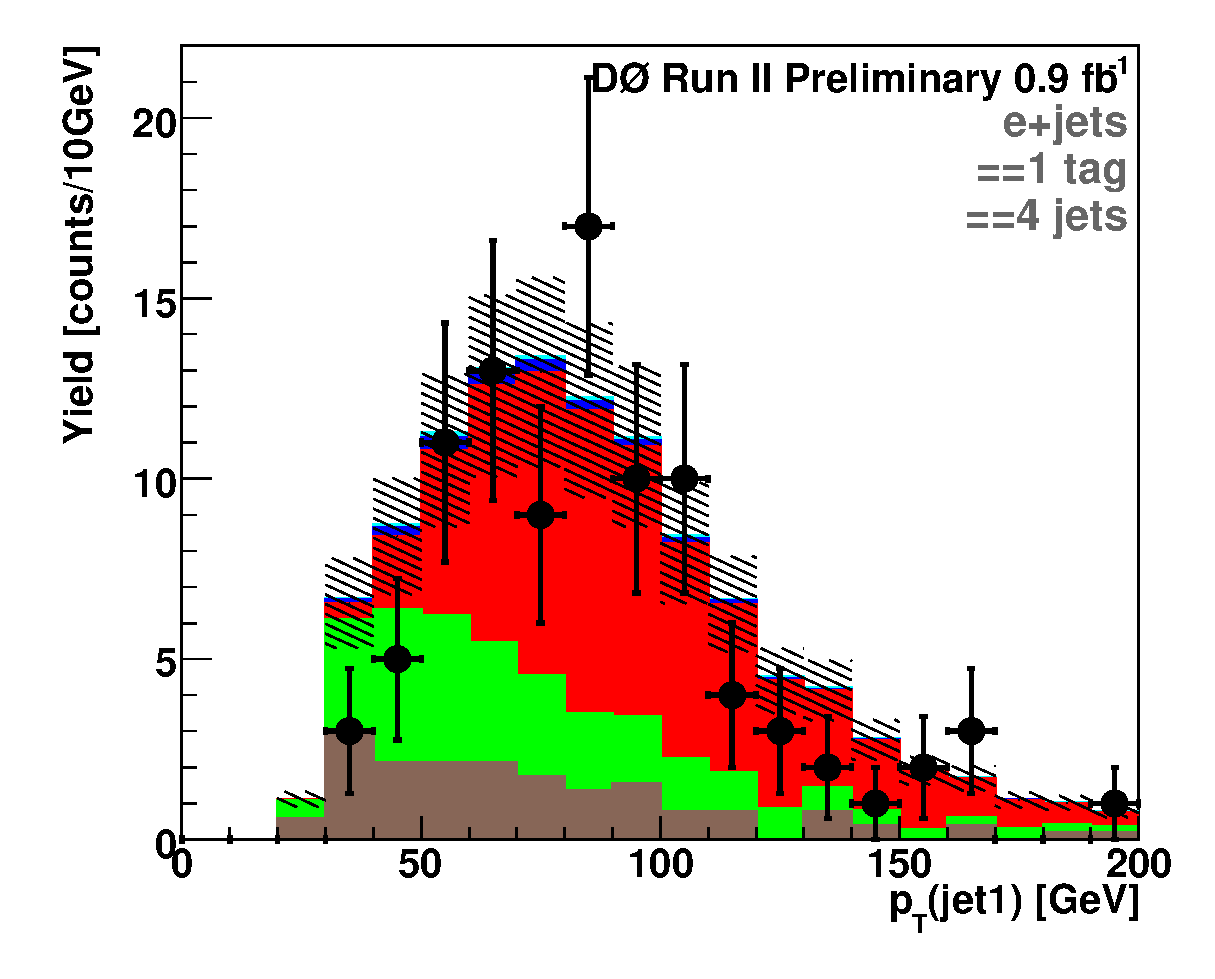
\includegraphics[width=0.32\textwidth]{eps/DataBackground/electron/CC_EqOneTag_EqFourJet_Jet1Pt.eps}
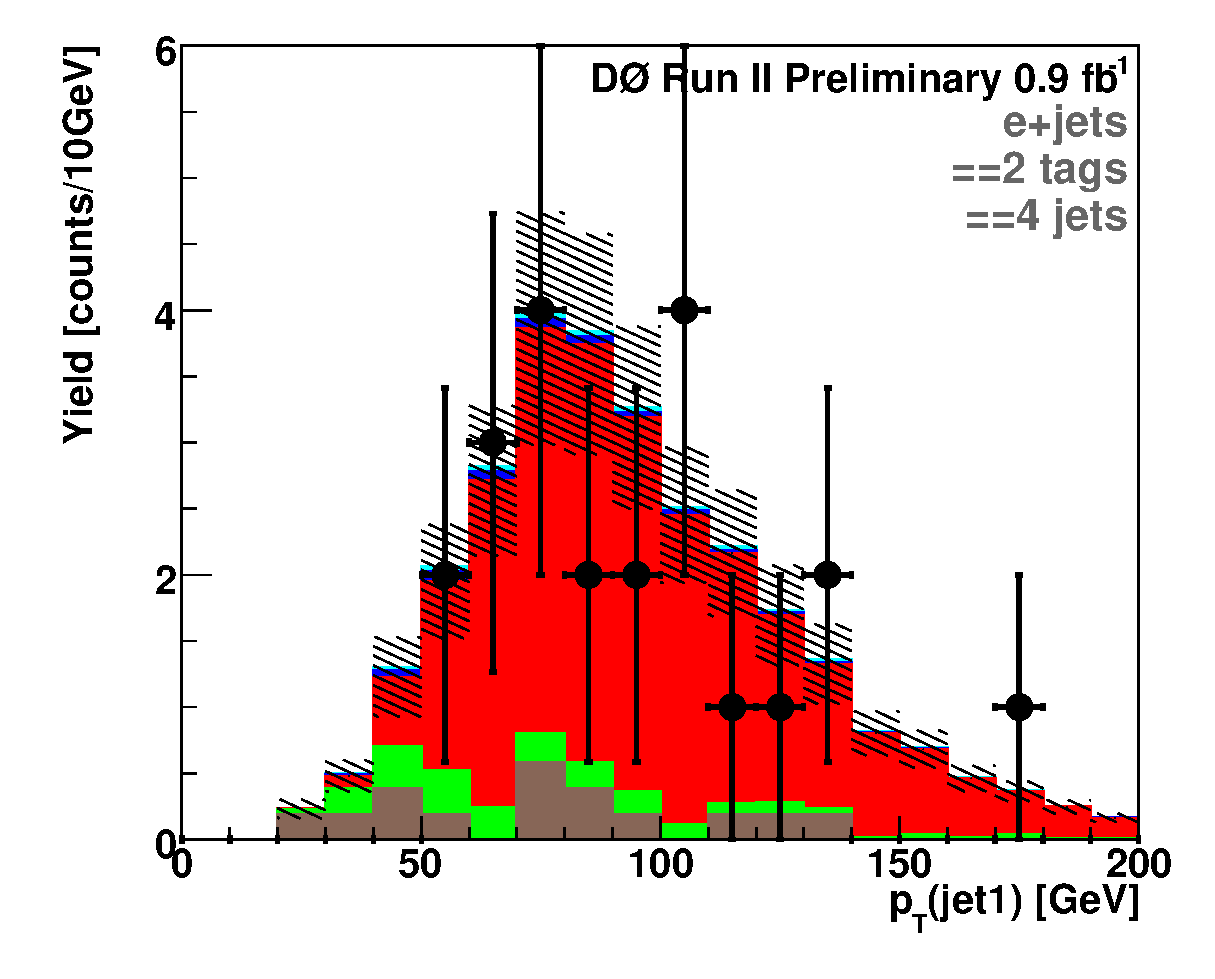
\includegraphics[width=0.32\textwidth]{eps/DataBackground/electron/CC_EqTwoTag_EqFourJet_Jet1Pt.eps}
\end{center}
\vspace{-0.1in}
\caption{Example leading order Feynman diagram for a ``W+jets" event. This particular diagram represents a strange quark and gluon collision production a W boson, one charm quark and a gluon.}
\label{wjets}
\end{figure}

